\chapter{Results}
\label{chap:results}
\begin{spacing}{1.5}

This chapter presents the results with regard to the evaluation of the RAG QA system across its two stages of development: the prototype and the full-scale implementation. 

Each followed a distinct evaluation protocol. For the prototype, responses were assessed through a dual strategy combining human annotation on a 5-point Likert scale -- measuring consistency, fluency, completeness, and relevance -- with automatic scoring from an external LLM (GPT-3.5), prompted as an evaluator. By contrast, the re-engineered system was tested on a synthetic collection of 508 single-hop and 908 combined queries automatically generated from the GNA operative manual. The assessment included intrinsic IR metrics -- Recall@, MRR, nDCG@, AP@, Latency --  to quantify retrieval performance, alongside qualitative human feedback, to capture user-facing quality. Feedback was collected systematically through in-interface ratings tasks: each response was labelled on a 3-point Likert scale -- 1 star equals ``poor'', 2 stars equals ``fair'', 3 stars equals ``good'' --, offering direct insight into the perceived relevance, completeness, and fluency of the generated answers.


\section{Prototyping Phase}
The prototype offered an initial proof of concept, validating that a RAG architecture could be applied to the GNA corpus. Although limited in scale, it provided important insights into feasibility.

The evaluation outcomes (\autoref{fig:proto_results}) show a clear profile: consistency was rated at the highest level ($\approx$ 5), indicating that generated answers rarely contradicted themselves. Relevance ($\approx$ 4.7) and fluency ($\approx$ 4.9) also scored strongly, confirming the system’s ability to generate both accurate and linguistically natural responses. Completeness, however, achieved slightly lower values ($\approx$ 4.6), pointing to occasional gaps in coverage where answers did not fully integrate all available evidence.

Performance testing further revealed practical constraints. Embedding generation averaged 31.2 seconds per batch, while query responses were returned in $\approx$ 1.26 seconds on average. While the latter figure was adequate for interactive use, efficiency lagged behind production-ready deployments, especially under load. 

In sum, the prototype confirmed the viability of a RAG-based QA approach, but also highlighted the need for more scalable retrieval infrastructure.

\begin{figure}[H]
  \centering
  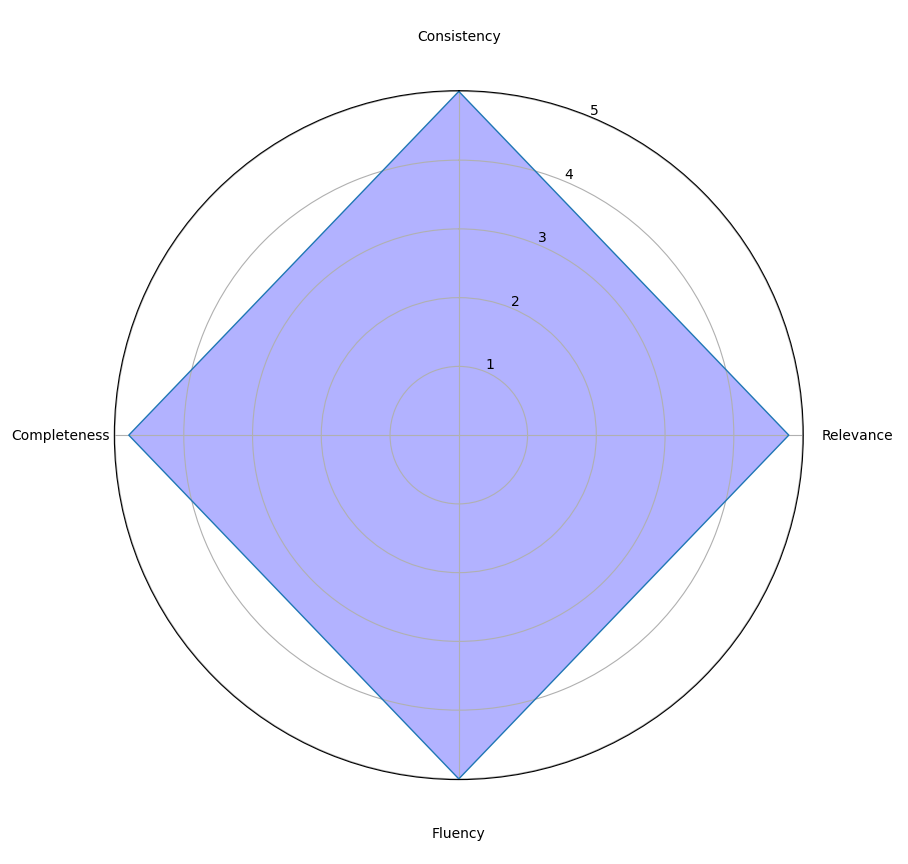
\includegraphics[width=\textwidth]{images/radar.png} 
  \caption{Evaluation results for prototype version of the GNA QA system.}
  \label{fig:proto_results}
\end{figure}


\section{Retrieval Performance and Ablation Studies}\label{sec:retrieval_ablation}
Retrieval performance pertinent to the full-scale system implementation was benchmarked in the experimental setup across different strategies: Dense, BM25, and Hybrid variants, with optional query rewriting and cross-encoder reranking. All runs were evaluated with @5 cut-offs -- R@5, MRR, nDCG@5, AP@5 --, complemented by latency measurements (seconds per query). This setup enables a consistent comparison of coverage, ranking quality, and efficiency across methods. The benchmarked retrieval scores and the different configurations tested are summarised in \autoref{tab:benchmark}.\\

\noindent The findings highlight distinct trade-offs across retrieval methods, presented hereafter.\\

\noindent \textbf{Single-hop dataset.}\\
The best overall performance was achieved by the \textbf{Hybrid + Score-blend} method without query rewriting and reranking (R@5 = 70.27, MRR = 48.59, nDCG@5 = 54.02, AP@5 = 48.59), with latency around 0.55 s. This configuration consistently outperformed \textbf{Dense} retriever -- the system’s initial baseline -- and \textbf{BM25} alone, showing the benefits of combining lexical and semantic signals. A close second was \textbf{Hybrid + Weighted RRF} (R@5 = 69.68, nDCG@5 = 52.49) at slightly lower latency (0.33 s).
\textbf{BM25} without extras proved a strong baseline (R@5 = 65.15) and remained by far the fastest method ($\approx$ 0.001 s), though it lagged behind hybrids in ranking quality. \textbf{Dense} retrieval showed competitive early-rank placement (MRR = 47.04) but lower recall and nDCG, confirming its limits when used in isolation.\\

\noindent \textbf{Combined(single-hop + multi-hop).}\\
Here, absolute scores dropped due to the increased complexity of multi-hop queries and the @5 cutoff, but the relative ordering of methods remained stable. \textbf{Hybrid + Score-blend} again provided the best balance, with R@5 = 55.35 and AP@5 = 36.69 at 0.45 s. \textbf{BM25} retained an edge in precision at early ranks (MRR = 51.23, nDCG@5 = 57.13), again with negligible latency ($\approx$ 0.001 s). \textbf{Hybrid + Weighted RRF} was also competitive (R@5 = 53.98, nDCG@5 = 56.92). \textbf{Dense} retrieval remained faster than hybrids (0.19-0.82 s) but less effective overall.\\

\noindent \textbf{Effect of rewriting and reranking.}\\
Across all methods, adding query rewriting or reranking consistently reduced effectiveness and inflated latency. Reranking with the MS-MARCO English cross-encoder reordered Italian, domain-specific candidates sub-optimally, while rewriting perturbed terminology that BM25 depends on. In practice, this meant added latency (up to 10 s in BM25 with rerank) and systematically lower recall and precision.\\

\noindent \textbf{Latency-quality trade-offs.}
\begin{itemize}
  \item Fastest: BM25 without extras (\~0.001 s);
  \item Best balance: Hybrid + Score-blend without extras (\~0.45-0.55 s), combining top recall and ranking quality with sub-second latency;
  \item Worst cost–benefit: query rewriting and reranking, which added seconds of latency without gains in retrieval quality.
\end{itemize}


\begin{table}[H]
\centering
\resizebox{\linewidth}{!}{%
\setlength{\tabcolsep}{3pt}
\footnotesize
\begin{tabular}{l c c *{10}{c}} % Method, Query rewrite, Rerank, then 10 numeric columns
\toprule
& & & \multicolumn{5}{c}{\textbf{SINGLE-HOP}} & \multicolumn{5}{c}{\textbf{COMBINED (single+multi-hop)}} \\
\cmidrule(lr){4-8}\cmidrule(lr){9-13}
\textbf{Method} & \shortstack[c]{\textbf{Query}\\\textbf{rewrite}} & \textbf{Rerank} & R@5 & MRR & nDCG@5 & AP@5 & Latency & R@5 & MRR & nDCG@5 & AP@5 & Latency \\
\midrule
Dense   &  \xmark     & \xmark & 67.51 & \underline{47.04} & 52.18 & \underline{47.04} & \underline{0.29}  & 50.78 & 48.21 & 53.70 & 34.98 & \underline{0.19} \\
        &  \checkmark & \xmark & 58.07 & 36.76 & 42.09 & 36.76 & 5.98 & 42.64 & 35.41 & 41.32 & 26.24 & 3.10   \\
        & \xmark      &  \checkmark  & 45.47 & 25.41 & 30.36 & 25.41 & 1.30  & 34.57 & 27.71 & 32.90 & 19.48 & 0.82 \\
        & \checkmark  &  \checkmark  & 52.55 & 31.66 & 36.87 & 31.66 & 4.76 & 38.16 & 30.45 & 36.0 & 22.51 & 3.46     \\
\addlinespace
BM25                          & \xmark & \xmark & 65.15 & 43.56 & 48.98 & 43.56 & \textbf{0.001} & 53.09 & \textbf{51.23} & \textbf{57.13} & 35.50 & \textbf{0.001} \\
                              & \checkmark & \xmark & 57.87 & 37.37 & 42.50 & 37.37 & 1.98 & 46.65 & 42.15 & 48.33 & 29.38 & 1.20     \\
                              & \xmark      &  \checkmark  & 45.47 & 25.41 & 30.36 & 25.41 & 1.30  & 34.57 & 27.71 & 32.90 & 19.48 & 0.82 \\
                              & \checkmark  &  \checkmark  & 43.89 & 25.87 & 30.35 & 25.87 & 10.02 & 35.18 & 30.33 & 35.68 & 20.59 & 4.96     \\
Hybrid                        &          &  &  &  &  &  &  &  &  &  &  &      \\
\hspace{0.5em}\textit{+ Weighted RRF}          & \xmark   & \xmark & \underline{69.68} & 46.72 & \underline{52.49} & 46.72 & 0.33  & \textbf{53.98} & \underline{50.93} & \underline{56.92} & \underline{36.15} & 0.32 \\
                              & \checkmark & \xmark & 57.48 & 37.48 & 42.48 & 37.48 & 4.38  & 43.52 & 38.41 & 44.10 & 27.68 & 3.21     \\
                              & \xmark      &  \checkmark  & 43.50 & 24.70 & 29.33 & 24.70 & 1.67  & 33.06 & 26.36 & 31.26 & 18.70 & 0.87 \\
                              & \checkmark  &  \checkmark  & 38.58 & 21.14 & 25.47 & 21.14 & 6.51 & 29.98 & 23.95 & 28.66 & 16.44 & 6.75     \\
\addlinespace
\hspace{0.5em}\textit{+ Score-blend}   & \xmark   & \xmark & \textbf{70.27} & \textbf{48.59} & \textbf{54.02} & \textbf{48.59} & 0.55 & \underline{53.35} & 50.84 & 56.48 & \textbf{36.69} & 0.45     \\
                              & \checkmark & \xmark & 57.67 & 37.17 & 42.31 & 37.17 & 4.57 & 43.61 & 38.16 & 43.87 & 27.52 & 3.99   \\
                              & \xmark      &  \checkmark  & 43.70 & 24.89 & 29.53 & 24.89 & 2.64 & 33.14 & 26.21 & 31.14 & 18.70 & 1.22   \\
                              & \checkmark  &  \checkmark  & 38.58 & 21.47 & 25.72 & 21.47 & 6.44 & 30.13 & 23.98 & 28.82 & 16.55 & 4.8   \\
\bottomrule
\end{tabular}%
}
\caption{Results for different retrieval methods on the test datasets. Best per column is bold and the second-best is underlined. Latency is measured in seconds per query. Reranking is performed using the \textit{cross-encoder/ms-marco-MiniLM-L-6-v2} model.}
\label{tab:benchmark}
\end{table}


\section{Qualitative Analysis}
The re-engineered system was evaluated not only through intrinsic metrics but also via direct user feedback, providing a complementary perspective on performance. As shown in \autoref{fig:ratings_}, user ratings distributed as follows: 65\% of answers received 3 stars (``Good''), 25\% received 2 stars (``Fair''), and 10\% received 1 star (``Poor'').


\begin{figure}[H]
  \centering
  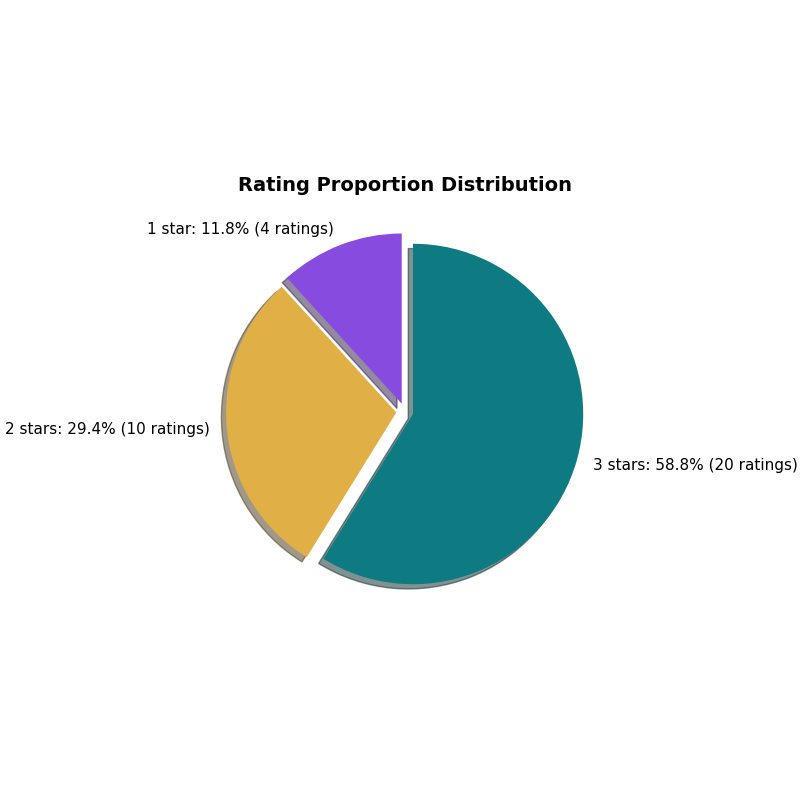
\includegraphics[width=\textwidth]{images/rating_proportions.png} 
  \caption{Distribution of user feedback ratings, showing the proportion of responses evaluated as poor (1 star), fair (2 stars), and good (3 stars).}
  \label{fig:ratings_}
\end{figure}

Instances of lower relevance were generally linked to ambiguous queries or to cases where vector sparsity limited the number of retrieved chunks. Despite these shortcomings, users highlighted several strengths: the system’s multilingual capabilities, the user-friendly interface, and the attempt to provide traceability through citations -- though, as discussed in \autoref{chap:discussion}, the citation mechanism requires further refinement.

Edge-case testing yielded additional insights. For out-of-domain queries, the system largely succeeded in avoiding hallucinations by producing cautious fallback responses. For example, (\autoref{fig:edge-case}), illustrates a query about contemporary art exhibitions in Rome: although the reply is incomplete and does not provide relevant content to the query, it faithfully reflects the system prompt’s instruction to refrain from answering questions outside the GNA scope, instead redirecting the user to the knowledge base.

Equally instructive were the tests on HTML snippets retrieval, a particular feature of the GNA user manual where HTML tags are embedded as procedural instructions for formatting reports. In these cases, the assistant correctly surfaced and rendered the relevant code blocks (see \autoref{fig:edge-case_code}), preserving both syntax and explanatory context. This demonstrated the system’s capacity to handle heterogeneous content types aside from plain text, thus addressing one of the distinctive characteristics of the GNA documentation.

Overall, the feedback evaluation demonstrates the feasibility and effectiveness of a RAG pipeline tailored to the GNA corpus. The prototype established proof of concept, while the full-scale implementation improved retrieval robustness and scalability. Although some challenges persist -- particularly with completeness, citation reliability, and response latency under reranking -- the system consistently produced relevant, fluent, and context-aware answers, confirming its potential as a practical assistant for navigating the GNA documentation.

\vspace{0.5em}
\begin{figure}[H]
  \centering
  
\includegraphics[width=\textwidth]{images/edge_case_response.png} 
  \caption{Edge case test of the GNA AI Assistant, showing an out-of-domain query about contemporary art exhibitions in Rome and the system’s fallback response with redirection to the GNA knowledge base.}
  \label{fig:edge-case}
\end{figure}

\begin{figure}[H]
  \centering
  
\includegraphics[width=\textwidth]{images/risposta_assistente_con_codice.png} 
  \caption{Example of the GNA QA system retrieving and presenting HTML code snippets from the knowledge base.}
  \label{fig:edge-case_code}
\end{figure}


\end{spacing}